\documentclass{standalone}
\usepackage{tikz}
\usetikzlibrary{calc}

\begin{document}
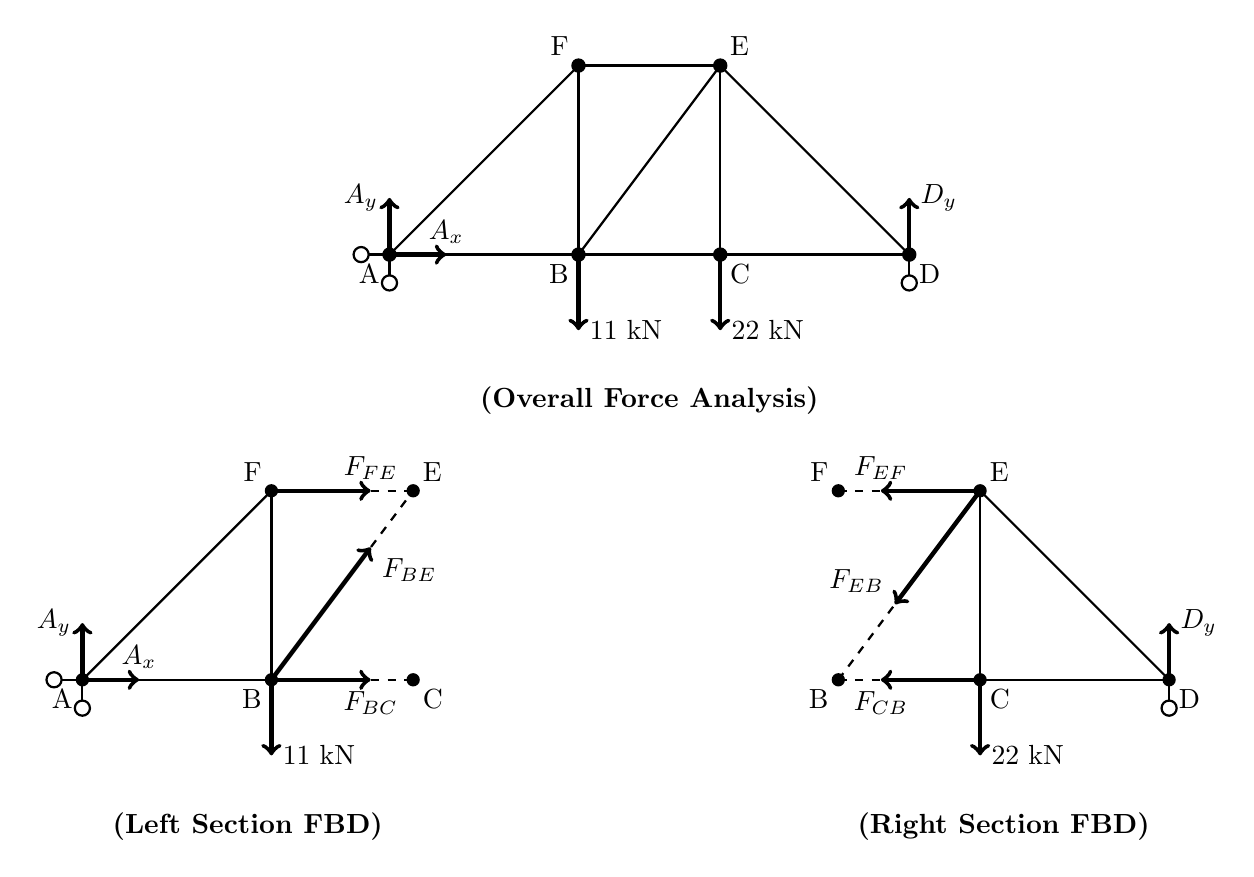
\begin{tikzpicture}[scale=1.2]
    % 受力分析 - 最上方居中
    \begin{scope}[yshift=4cm, xshift=3.25cm]
    % 定义节点坐标
    \coordinate (A) at (0, 0);      % 左支座点A
    \coordinate (B) at (2, 0);      % 节点B  
    \coordinate (C) at (3.5, 0);    % 节点C
    \coordinate (D) at (5.5, 0);    % 右支座点D
    \coordinate (E) at (3.5, 2);    % 上弦节点E
    \coordinate (F) at (2, 2);      % 上弦节点F
    
    % 绘制桁架构件
    \draw[thick] (A) -- (B) -- (C) -- (D);  % 下弦
    \draw[thick] (F) -- (E);                % 上弦
    \draw[thick] (A) -- (F);                % 左端斜杆
    \draw[thick] (B) -- (F);                % BF杆
    \draw[thick] (B) -- (E);                % BE杆
    \draw[thick] (C) -- (E);                % CE杆
    \draw[thick] (E) -- (D);                % ED杆
    
    % 绘制节点
    \fill (A) circle (2pt) (B) circle (2pt) (C) circle (2pt) 
                 (D) circle (2pt) (E) circle (2pt) (F) circle (2pt);
    \draw (A) circle (2pt) (B) circle (2pt) (C) circle (2pt) 
          (D) circle (2pt) (E) circle (2pt) (F) circle (2pt);
    
    % 节点标签
    \node[below left] at (A) {A};
    \node[below left] at (B) {B};
    \node[below right] at (C) {C};
    \node[below right] at (D) {D};
    \node[above right] at (E) {E};
    \node[above left] at (F) {F};
    
    % 支座
    % A点固定支座
    \draw[thick] (A) -- +(0,-0.3);  % 垂直向下的短线段
    \draw[thick, fill=white] (A) +(0,-0.3) circle (0.08);  % 底部白色圆圈
    \draw[thick] (A) -- +(-0.3,0);  % 水平向左的短线段
    \draw[thick, fill=white] (A) +(-0.3,0) circle (0.08);  % 左侧白色圆圈
    
    % D点铰支座
    \draw[thick] (D) -- +(0,-0.3);  % 垂直向下的短线段
    \draw[thick, fill=white] (D) +(0,-0.3) circle (0.08);  % 底部白色圆圈
    
    % 载荷
    % B点载荷 11kN
    \draw[->, black, ultra thick] (B) -- +(0,-0.8) node[right] {11 kN};
    
    % C点载荷 22kN  
    \draw[->, black, ultra thick] (C) -- +(0,-0.8) node[right] {22 kN};
    
    % 支反力
    % A点支反力
    \draw[->, black, ultra thick] (A) -- +(0,0.6) node[left] {$A_y$};  % A_y向上
    \draw[->, black, ultra thick] (A) -- +(0.6,0) node[above] {$A_x$}; % A_x向右
    
    % D点支反力
    \draw[->, black, ultra thick] (D) -- +(0,0.6) node[right] {$D_y$}; % D_y向上
    
    % 图片标题
    \node[below] at (2.75,-1.3) {\textbf{(Overall Force Analysis)}};
    \end{scope}

    % 左截面图形 - 左下方
    \begin{scope}[yshift=-0.5cm]
    % 定义节点坐标
    \coordinate (LA) at (0, 0);      % 左支座点A
    \coordinate (LB) at (2, 0);      % 节点B  
    \coordinate (LC) at (3.5, 0);    % 节点C
    \coordinate (LE) at (3.5, 2);    % 上弦节点E
    \coordinate (LF) at (2, 2);      % 上弦节点F

    % 节点标签
    \node[below left] at (LA) {A};
    \node[below left] at (LB) {B};
    \node[below right] at (LC) {C};
    \node[above right] at (LE) {E};
    \node[above left] at (LF) {F};

    % 绘制节点(实心圆)
    \fill (LA) circle (2pt) (LB) circle (2pt) (LC) circle (2pt) 
          (LE) circle (2pt) (LF) circle (2pt);

    % 绘制桁架构件
    \draw[thick] (LA) -- (LB);  % 下弦AB段
    \draw[thick, dashed] (LB) -- (LC);  % 下弦BC段(被截断,虚线)
    \draw[thick, dashed] (LF) -- (LE);  % 上弦EF段(被截断,虚线)
    \draw[thick] (LA) -- (LF);                % 左端斜杆
    \draw[thick] (LB) -- (LF);                % BF杆
    \draw[thick, dashed] (LB) -- (LE);        % BE杆(被截断,虚线)

    % 支座
    % A点固定支座
    \draw[thick] (LA) -- +(0,-0.3);  % 垂直向下的短线段
    \draw[thick, fill=white] (LA) +(0,-0.3) circle (0.08);  % 底部白色圆圈
    \draw[thick] (LA) -- +(-0.3,0);  % 水平向左的短线段
    \draw[thick, fill=white] (LA) +(-0.3,0) circle (0.08);  % 左侧白色圆圈
    
    % 载荷和支反力
    % B点载荷 11kN
    \draw[->, black, ultra thick] (LB) -- +(0,-0.8) node[right] {11 kN};
    
    % A点支反力
    \draw[->, black, ultra thick] (LA) -- +(0,0.6) node[left] {$A_y$};  % A_y向上
    \draw[->, black, ultra thick] (LA) -- +(0.6,0) node[above] {$A_x$}; % A_x向右
    
    % 截面内力
    % F_FE (作用点在F,指向E)
    \draw[->, black, ultra thick] (LF) -- +($0.7*(LE) - 0.7*(LF)$) node[above] {$F_{FE}$};
    
    % F_BE (作用点在B,指向E)  
    \draw[->, black, ultra thick] (LB) -- +($0.7*(LE) - 0.7*(LB)$) node[below right] {$F_{BE}$};
    
    % F_BC (作用点在B,指向C)
    \draw[->, black, ultra thick] (LB) -- +($0.7*(LC) - 0.7*(LB)$) node[below] {$F_{BC}$};
    
    % 图片标题
    \node[below] at (1.75,-1.3) {\textbf{(Left Section FBD)}};
    \end{scope}
    
    % 右截面图形 - 右下方
    \begin{scope}[xshift=6cm, yshift=-0.5cm]
    % 定义节点坐标
    \coordinate (RB) at (2, 0);      % 节点B  
    \coordinate (RC) at (3.5, 0);    % 节点C
    \coordinate (RD) at (5.5, 0);    % 右支座点D
    \coordinate (RE) at (3.5, 2);    % 上弦节点E
    \coordinate (RF) at (2, 2);      % 上弦节点F

    % 节点标签
    \node[below left] at (RB) {B};
    \node[below right] at (RC) {C};
    \node[below right] at (RD) {D};
    \node[above right] at (RE) {E};
    \node[above left] at (RF) {F};

    % 绘制节点(实心圆)
    \fill (RB) circle (2pt) (RC) circle (2pt) 
          (RD) circle (2pt) (RE) circle (2pt) (RF) circle (2pt);

    % 绘制桁架构件
    \draw[thick, dashed] (RB) -- (RC);  % 下弦BC段(被截断,虚线)
    \draw[thick] (RC) -- (RD);  % 下弦CD段
    \draw[thick, dashed] (RF) -- (RE);  % 上弦EF段(被截断,虚线)
    \draw[thick, dashed] (RB) -- (RE);  % BE杆(被截断,虚线)
    \draw[thick] (RC) -- (RE);                % CE杆
    \draw[thick] (RE) -- (RD);                % ED杆

    % 支座
    % D点铰支座
    \draw[thick] (RD) -- +(0,-0.3);  % 垂直向下的短线段
    \draw[thick, fill=white] (RD) +(0,-0.3) circle (0.08);  % 底部白色圆圈
    
    % 载荷和支反力
    % C点载荷 22kN  
    \draw[->, black, ultra thick] (RC) -- +(0,-0.8) node[right] {22 kN};
    
    % D点支反力
    \draw[->, black, ultra thick] (RD) -- +(0,0.6) node[right] {$D_y$}; % D_y向上
    
    % 截面内力
    % F_EF (作用点在E,指向F)
    \draw[->, black, ultra thick] (RE) -- +($0.7*(RF) - 0.7*(RE)$) node[above] {$F_{EF}$};
    
    % F_EB (作用点在E,指向B)  
    \draw[->, black, ultra thick] (RE) -- +($0.6*(RB) - 0.6*(RE)$) node[above left] {$F_{EB}$};
    
    % F_CB (作用点在C,指向B)
    \draw[->, black, ultra thick] (RC) -- +($0.7*(RB) - 0.7*(RC)$) node[below] {$F_{CB}$};
    
    % 图片标题
    \node[below] at (3.75,-1.3) {\textbf{(Right Section FBD)}};
    \end{scope}

\end{tikzpicture}
\end{document}
